\section[Controllo centralizzato ai giunti]{Controllo centralizzato ai giunti \\ \small \textit{Centralized Joint Space Control}}

In alcuni casi il \textbf{controllo decentralizzato} a giunti indipendenti \textbf{può risultare inadeguato}. Questo accade, ad esempio, quando:
\begin{itemize}
	\item sono \textbf{richieste velocità operative elevate} $\implies$ le coppie di disturbo strutturato dipendenti dalla velocità (di Coriolis, centrifughe) influiscono pesantemente sul comportamento dei giunti
	\item i \textbf{motori sono ad azione diretta} $\implies$ a causa dell’assenza dei motoriduttori ($\mathbf{K}_r = \mathbf{I}$) non si beneficia di alcuna riduzione degli effetti non lineari e di accoppiamento fra i giunti
\end{itemize}
 
In tali casi gli effetti delle coppie di disturbo $\mathbf{d}$ possono determinare errori troppo elevati di inseguimento della traiettoria.
 
Poiché in questi casi non è possibile ridurre sufficientemente gli effetti indotti dalle coppie di disturbo $\mathbf{d}$, diventa conveniente cercare di eliminare direttamente tali coppie, ricorrendo ad una \textbf{strategia di controllo contenente termini non lineari di compensazione}.\\
Si parla di \textbf{controllo centralizzato} perché la coppia applicata a ciascun giunto risulta funzione anche delle variabili di posizione e velocità degli altri giunti, a differenza di quanto accade nel controllo a giunti indipendenti.
 
Negli schemi di controllo centralizzato il manipolatore è considerato come un \textbf{unico sistema MIMO}, con n ingressi (le coppie applicate ai giunti) e n uscite (le posizioni dei giunti) che interagiscono fra loro secondo relazioni non lineari. La \textbf{legge di controllo} centralizzato dovrà tenere conto del modello dinamico del manipolatore ed essere \textbf{non-lineare} (visto che il modello è non lineare).
 
 
 
\subsubsection{Idea principale}
Il principale approccio di controllo centralizzato è detto a \textbf{dinamica inversa}, perché la coppia di comando è ricavata dall’equazione dinamica del manipolatore a partire dalla conoscenza delle variabili giunto (posizioni e velocità), ovvero dalla risoluzione del problema della dinamica inversa.\\
Ovvero usando il modello dinamico:
\boldmath
$$
B(q)\ddot{q} + C(q, \dot{q})\dot{q} + F_v\dot{q} + g(q) = \tau
$$
\unboldmath

ci calcoliamo $\boldsymbol{\tau}$, che poi andiamo a fornire ai nostri attuatori, che quindi in questo caso saranno in modalità \textbf{torque-controlled}.




\subsubsection{Ora usiamo attuatori torque-controlled}
Come accennato in questo caso abbiamo bisogno di generatori di coppia.

Richiamando la forma semplificata del bilancio elettrico di armatura (\ref{eq:simplified_armature_electrical_balance}), possiamo scrivere:
$$
I_a = R_a^{-a}(V_a - K_\omega \omega_m) = R_a^{-1}(G_vV_c - K_\omega \omega_m)
$$
Dove l'ultima ugualianza deriva dall'amplificatore di potenza: $V_a = G_v V_c$.
Di conseguenza, ricordando (sempre al modello del motore: vedi fig. \ref{fig:electricactuator1}), che $\tau_m = K_t I_a$, possiamo scrivere:
$$
\tau = K_r \tau_m = K_r K_t I_a = K_r K_t R_a^{-1}(G_vV_c - K_\omega \omega_m)
$$
che si può notare essere uguale a (\ref{eq:torque_command}).

Visto che però vogliamo avere un motore torque-controlled (come possiamo ricordare) è necessario inserire la corrente in retroazione. Per magimagia (forse vedi sezione \ref{section:torque_generator}) diciamo che il termine con $K_\omega$ diventa trascurabile e quindi:
$$
I_a = R_a^{-1}(G_vV_c) = G_i V_c
$$
Di conseguenza
\boldmath
$$
\tau = K_r K_t G_i V_c = u
$$
\unboldmath
ove $\mathbf{u}$ è il vettore di comandi disponibili per il controllo.








\subsection{Controllo a dinamica inversa}
L’approccio di controllo a dinamica inversa è basato sull’idea di ottenere una \textbf{linearizzazione della dinamica del sistema per mezzo di una retroazione non lineare} degli stati tale da condurre ad un sistema lineare e disaccoppiato rispetto ad un nuovo vettore di accelerazioni di comando da progettare. Ovvero utilizzamo la tecnica nota come \textbf{feedback linearization}.

Prima di cominciare, per comodità definiamo il modello della dinamica come:
\boldmath
\begin{equation}\label{eq:simplified_notation_dynamic}
B(q)\ddot{q} + n(q, \dot{q}) = \tau = u
\end{equation}
dove:
$$
n(q, \dot{q}) \triangleq C(q, \dot{q})\dot{q} + F_v\dot{q} + g(q)
$$
\unboldmath

Supponendo di poter calcolare esattamente $\mathbf{B(q)}$ e $\mathbf{n(q, \dot{q})}$, definiamo il nostro comando di controllo come
\boldmath
$$
u = B(q)y + n(q, \dot{q})
$$
questo perchè, così facendo, riusciamo ad ottenere una \textbf{linearizzazione esatta del sistema}:
\begin{gather*}
B(q)\ddot{q} + \cancel{n(q, \dot{q})} = \tau = u = B(q)y + \cancel{n(q, \dot{q})} \\
\Updownarrow \\
\cancel{B(q)}\ddot{q} = \cancel{B(q)}y \\
\Updownarrow \\
\ddot{q} = y
\end{gather*}
Il sistema risultante è costituito da n doppi integratori: la i-esima componente $y_i$ del nuovo comando influenza solo il comportamento della i-esima coordinata giunto $q_i$, che risulta indipendente dal moto degli altri giunti.


\begin{figure}[H]
	\centering
	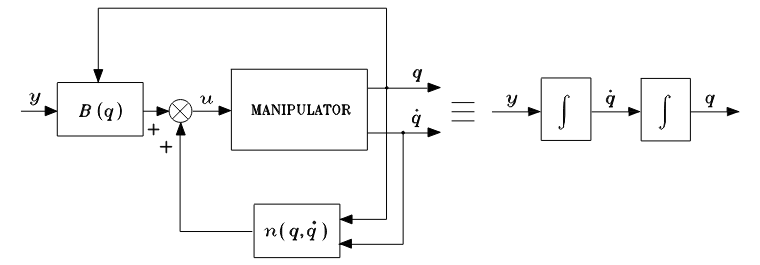
\includegraphics[width=0.8\linewidth]{images/centralized_control_1}
	\caption{Feedback linearization}
	\label{fig:centralizedcontrol1}
\end{figure}

La scelta più semplice per il nuovo comando $\mathbf{y}$ è data da una legge di \textbf{controllo di tipo PD}:
$$
y = -K_P q - K_D \dot{q} + r
$$

che quindi, sostituiendo a $\ddot{q} = y$, otteniamo il seguente sistema di equazioni del secondo ordine:
\begin{equation}\label{eq:2nd_order_dyn_feedback_lin}
\ddot{q} + K_D \dot{q} + K_P q = r
\end{equation}
asintoticamente stabile se le matrici $K_P$ e $K_D$ sono definite positive.
Scegliendo in particolare $K_P$ e $K_D$ diagonali, il sistema rimane disaccoppiato e ad ogni variabile giunto viene assegnata la dinamica corrispondente ai guadagni imposti con:
\unboldmath
$$
\mathbf{K_P} = diag\{\omega_{n1}^2, \ \dots, \ \omega_{nn}^2\}
\quad
\mathbf{K_D} = diag\{2\zeta\omega_{n1}, \ \dots, \ 2\zeta\omega_{nn}^2\}
$$

\boldmath
Il vettore di riferimento $r$ è definito a partire dalla traiettoria desiderata, pianificata ai giunti, come:
$$
r \triangleq \ddot{q}_d + K_D \dot{q}_d + K_P q_d 
$$
Possiamo ora analizzare la dinamica dell'errore di inseguimento, sostituendo la definizione di $r$ a (\ref{eq:2nd_order_dyn_feedback_lin}):
$$
(\ddot{q}_d - \ddot{q}) + K_D(\dot{q}_d - \dot{q}) + K_P(q_d - q) = 0
\implies
\ddot{e} + K_D\dot{e} + K_Pe = 0
$$
se $e(0) = 0$ e $\dot{e}(0) = 0$, l'errore converge a 0 con velocità e caratteristiche determinate da $K_P$ e $K_D$.
\unboldmath

Il sistema risultante è mostrato in fig. \ref{fig:centralizedcontrol2}, dove notiamo due anelli: quello più interno è l'anello di linearizzazione, mentre quello esterno è il controllo (ora lineare) del nostro sistema.

\begin{figure}
	\centering
	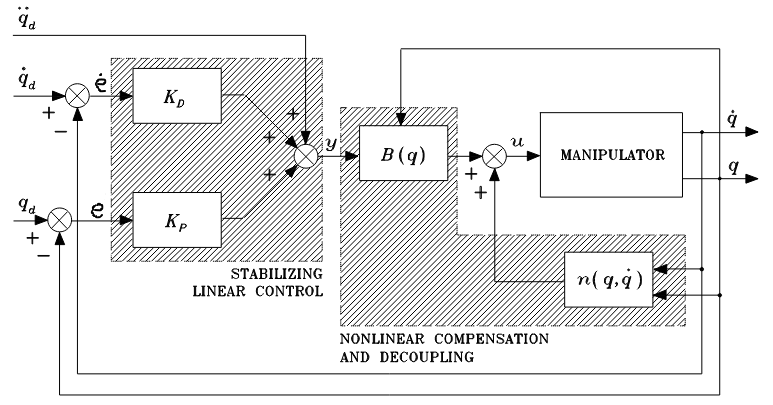
\includegraphics[width=0.7\linewidth]{images/centralized_control_2}
	\caption{Schema a blocchi del controllo a dinamica inversa nello spazio dei giunti}
	\label{fig:centralizedcontrol2}
\end{figure}


\vspace{20pt}
\subsubsection{Problemi}
L’ipotesi di linearizzazione esatta presuppone la capacità di calcolare \textit{online} le matrici $\mathbf{B(q)}$ e $\mathbf{n(q, \dot{q})}$ in modo esatto. Nella pratica però questo non è sempre possibile.
Per compensare a questi errori è necessario utilizzare altre tecniche, ad esempio algoritmi di controllo robusto.

Supponiamo di avere solo delle approssimazioni delle matrici, che chiameremo $\mathbf{\hat{B}(q)}$ e $\mathbf{\hat{n}(q, \dot{q})}$:
\boldmath
\begin{gather*}
B(q)\ddot{q} + n(q, \dot{q}) = \hat{B}(q)y + \hat{n}(q, \dot{q}) \\
\Updownarrow \\
\ddot{q} = B^{-1}\hat{B}y + B^{-1}(\hat{n} - n) \\
\Updownarrow \\
\ddot{q} = y + (B^{-1}\hat{B} - I)y + B^{-1}(\hat{n} - n) \\
\Updownarrow \\
\ddot{q} = y - \eta(q, \dot{q}, y) \\
\Downarrow \\
\ddot{e} + K_D\dot{e} + K_Pe = \eta(q, \dot{q}, y)
\end{gather*}

where
$$
\eta(q, \dot{q}, y) \triangleq (I - B^{-1}\hat{B})y - B^{-1}(\hat{n} - n)
$$

Il sistema ottenuto non è più lineare e disaccoppiato.

Per fortuna, \textbf{nella pratica}, il metodo della dinamica inversa \textbf{risulta abbastanza robusto} anche nel caso di linearizzazione approssimata, per cui viene usato sia senza ulteriori modifiche, sia con l’aggiunta di un termine robustificante.\\

\vspace{10pt}
\subsubsection{Vari schemi visti come dinamica inversa}
Tra gli schemi a dinamica inversa con linearizzazione approssimata, che non prevedono l’inserimento di termini robustificanti, possiamo includere:
\begin{itemize}
	\item \textbf{Controllo a giunti indipendenti}: questo approccio precedentemente analizzato può essere considerato come un caso particolare di controllo a dinamica inversa con linearizzazione approssimata, ottenuto ponendo:
	$$
	\hat{B}(q) = \bar{B} \quad , \quad \hat{n}(q, \dot{q}) = 0
	$$
	\item \textbf{Metodo della coppia calcolata} (o controllo a dinamica inversa in feedforward): già visto in sezione \ref{section:computed_torque}
	\item \textbf{Controllo PD con compensazione della gravità}, che vediamo nella prossima sezione; questo controllo può essere visto come dinamica inversa ponendo:
	$$
	\hat{B}(q) = I \quad , \quad \hat{n}(q, \dot{q}) = g(q)
	$$
\end{itemize}
\unboldmath









\subsection{Controllo PD con compensazione della gravità}

Nel caso in cui si voglia assegnare al manipolatore una \textbf{postura di equilibrio costante} (anziché una traiettoria completa), è possibile realizzare un controllore tale da garantire la stabilità asintotica globale di tale postura.

Facendo riferimento a (\ref{eq:simplified_armature_electrical_balance}): $B(q)\ddot{q} + n(q, \dot{q}) = u$, definiamo il controllo come:
\boldmath
$$
u \triangleq g(q) + K_P(q_d - q) - K_D\dot{q}
$$

Così facendo, sostituendo $u$ a (\ref{eq:simplified_armature_electrical_balance}), otteniamo:
\begin{equation}\label{eq:pd_gravity_comp_dyn}
B(q)\ddot{q} + C(q, \dot{q})\dot{q} + F_v\dot{q} + \cancel{g(q)} = \cancel{g(q)} + K_P(q_d - q) - K_D\dot{q}
\end{equation}

Ovvero si riescono a cancellare gli effetti della gravità.

\begin{figure}[H]
	\centering
	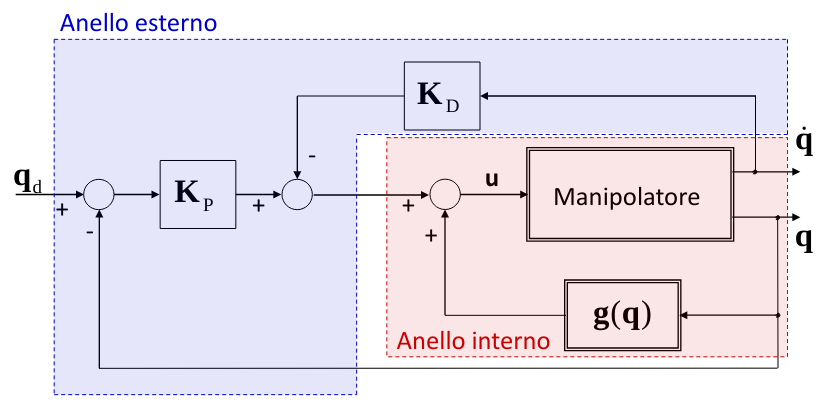
\includegraphics[width=0.6\linewidth]{images/centralized_control_pd_gravity_comp}
	\caption{Controllo PD con compensazione della gravità}
	\label{fig:centralizedcontrolpdgravitycomp}
\end{figure}
(notare che nel circuito non è presente $\dot{q}_d$: questo poichè essendo $q_d$ costante la sua derivata è nulla)

Analizzando il sistema risultante da (\ref{eq:pd_gravity_comp_dyn}), possiamo vedere che l'unico punto di equilibrio è dato da $q = q_d$:
\unboldmath
\begin{align*}
x \ \text{punto di equilibro} 
&\iff 
\dot{x} = \begin{pmatrix}\dot{q} \\ \ddot{q}\end{pmatrix} = 0
\stepcounter{equation}\tag{\theequation}\label{eq:pd_grav_comp_equil} \\
&\iff 
B(q)\cancelto{0}{\ddot{q}} + C(q, \dot{q})\cancelto{0}{\dot{q}} + F_v\cancelto{0}{\dot{q}} = K_P(q_d - q) - K_D\cancelto{0}{\dot{q}} \\
&\iff
0 = K_P(q_d - q) \\
&\iff
q = q_d
\end{align*}

Ovvero proprio quello che volevamo: stabilità in una postura costante $\mathbf{q}_d$.\\
Per fare un esempio, immagina il robot in figura \ref{fig:centralizedcontrolpdgravitycompexample}: il motori dovranno applicare delle coppie (i quali valori dipendono dal valore di $\mathbf{u}$ mostrato prima) per far rimanere il braccio in questa posizione statica.

\begin{figure}[H]
	\centering
	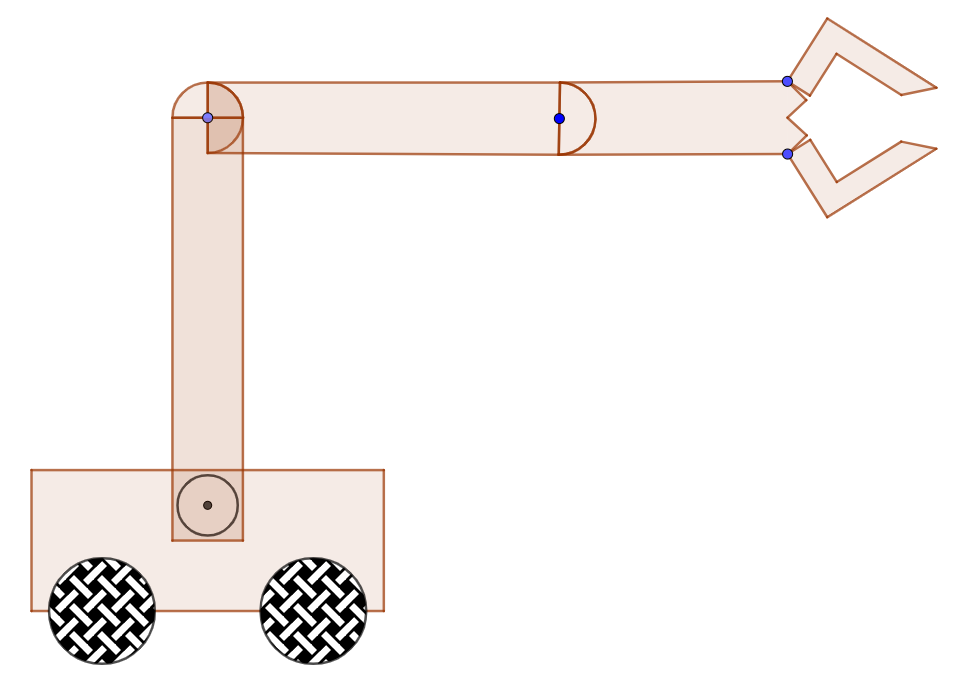
\includegraphics[width=0.5\linewidth]{images/centralized_control_pd_gravity_comp_example}
	\caption{Esempio di compensazione gravità}
	\label{fig:centralizedcontrolpdgravitycompexample}
\end{figure}




\vspace{20pt}
\subsubsection{Dimostrazione stabilità}
\boldmath
Per dimostrare le caratteristiche di stabilità del punto di equilibrio corrispondente alla postura desiderata, è possibile applicare il \textbf{metodo diretto di Lyapunov}. Definiamo $e \triangleq q_d - q$ e consideriamo come funzione di Lyapunov:
$$
V(\dot{q}, e) = \frac{1}{2}\dot{q}^TB(q)\dot{q} + \frac{1}{2}e^TK_Pe > 0    \qquad \forall q,e\neq0
$$
Dove possiamo interpretare il primo termine come l’energia cinetica del sistema ed il secondo come l’energia potenziale immagazzinata grazie alle rigidezze equivalenti date dai guadagni delle retroazioni delle posizioni ai giunti.

In questa funzione è stato scelto come stato del sistema il vettore $(e, \ \dot{q})^T$ che, dal punto di vista dell'equilibro, è equivalente a quanto usato in (\ref{eq:pd_grav_comp_equil}):
\begin{gather*}
\gamma \triangleq \begin{pmatrix}e \\ \dot{q}\end{pmatrix} = \begin{pmatrix}q - q_d \\ \dot{q}\end{pmatrix}
\implies 
\dot{\gamma} = \begin{pmatrix}\dot{e} \\ \ddot{q}\end{pmatrix} = \begin{pmatrix}\dot{q} - \cancelto{0}{\dot{q}_d} \\ \ddot{q}\end{pmatrix} = \begin{pmatrix}\dot{q} \\ \ddot{q}\end{pmatrix}
\end{gather*}



Ora passiamo allo studio del segno di $V$ lungo le traiettorie del sistema (come è richiesto dal metodo di Lyapunov). Derivando (ricordando che $\dot{q}_d = 0$, essendo $q_d$ costante), otteniamo:
$$
\dot{V} = \dot{q}^TB(q)\ddot{q} + \frac{1}{2}\dot{q}\dot{B}(q)\dot{q} - \dot{q}^TK_Pe
$$
procediamo sostituendo a $B(q)\ddot{q}$ la forma di esso fornita da (\ref{eq:pd_gravity_comp_dyn}) (ricordando la definizione di $e \triangleq q_d - q$):
\begin{gather*}
	B(q)\ddot{q} + C(q, \dot{q})\dot{q} + F_v\dot{q} = K_Pe - K_D\dot{q} \\
	\Updownarrow \\
	B(q)\ddot{q} = -C(q, \dot{q})\dot{q} - F_v\dot{q} + K_Pe - K_D\dot{q} \\
	\Downarrow \\
	\dot{V} = \dot{q}^T( -C(q, \dot{q})\dot{q} - F_v\dot{q} + \cancel{K_Pe} - K_D\dot{q} ) + \frac{1}{2}\dot{q}\dot{B}(q)\dot{q} - \dot{q}^T \cancel{K_Pe}
\end{gather*}

Raccogliendo i termini rimasti si ha
$$
\dot{V} = \frac{1}{2} \dot{q}^T ( \cancelto{0}{ \dot{B}(q) - 2C(q, \dot{q}) })\dot{q} - \dot{q}^T (F_v + K_D)\dot{q}
$$
dove la cancellazione a 0 è fatta grazie alla \textit{null-property} di quella differenza (si può dimostrare dalle equazioni della dinamica).

Allora:
$$
\dot{V} = - \dot{q}^T (F_v + K_D)\dot{q}
$$
che risulta essere \textbf{semi-definita negativa}. È solo \textbf{semi}-definita poichè è presente solo $\dot{q}$: $\dot{V} = 0$ per $\dot{q} = 0$ ma per qualsiasi $e$.

Possiamo però ora osservare che comunque $\dot{V} = 0 \iff \dot{q} = 0$, e di conseguenza anche $\ddot{q} = 0$. Ricordando da (\ref{eq:pd_grav_comp_equil}) che $(\dot{q}, \ddot{q}) = (0,0)$ è la condizione di equilibrio, possiaom dire che $\dot{V}$ si annulla solo per l'unico punto di equilibrio del sistema.
Dal teorema di \textit{La Salle-Krasowski} risulta pertanto globalmente asintoticamente stabile, come desiderato.
\unboldmath

\vspace{15pt}
\begin{addendum}
\textbf{Thm.} La Salle-Krasowski

Supponi che un sistema dinamico sia rappresentato da $\dot{\mathbf{x}}=f(\mathbf{x})$, dove $\mathbf{x}$ è il vettore dello stato e $f(\mathbf{0})=0$.\\
Se prendiamo una funzione $V$ tale che:
$$
\begin{cases}
	V(\mathbf{x}) > 0 \\
	\dot{V(\mathbf{x})} \leq 0
\end{cases}
$$
(i.e. $V$ positiva e $\dot{V}$ semi-definita negativa), \textbf{ma}
$$
\dot{V}(\mathbf{x}) = 0 \iff \mathbf{x} = 0
$$
allora abbiamo che l'\textbf{origine} $\mathbf{x} = 0$ è \textbf{asintoticamente stabile}.
\end{addendum}










\section{Controllo nello spazio operazionale}
La \textbf{traiettoria} desiderata da applicare al manipolatore è \textbf{spesso pianificata nello spazio operazionale}, mentre gli schemi di controllo analizzati finora sono tutti definiti nello spazio dei giunti.
\textbf{In tutti questi casi}, il riferimento di posizione ai giunti deve essere determinato a partire da quello cartesiano per mezzo della \textbf{cinematica inversa} (i riferimenti di velocità ed accelerazione sono spesso determinati per differenziazione numerica, dato che la cinematica inversa delle velocità e soprattutto delle accelerazioni può risultare troppo gravosa).

Una diversa soluzione al problema può essere trovata definendo lo \textbf{schema di controllo direttamente nello spazio operazionale} anziché in quello dei giunti. \\
Poiché le variabili disponibili (misurabili) sono quelle ai giunti (posizione ed eventualmente la velocità), è necessario in questo caso utilizzare la \textbf{cinematica diretta} per determinare le variabili cartesiane da confrontare con il riferimento desiderato. Si definiscono così anelli di controllo in retroazione in cui \textbf{l’inversione cinematica della traiettoria è sostituita dalla trasformazione delle coordinate}, racchiusa nell’anello di controllo stesso.

Tutti gli \textbf{schemi di controllo realizzati nello spazio operazionale sono “pesanti”} dal punto di vista computazionale: questo può portare a serie limitazioni sulla scelta del passo di campionamento e conseguentemente a degradate prestazioni del controllo. Nonostante questo, a differenza degli schemi di controllo nello spazio dei giunti (che sono solitamente idonei ad ottenere un buon controllo del moto), gli schemi di controllo nello spazio operazionale sono basilari nel caso in cui il manipolatore sia in \textbf{contatto con l’ambiente esterno} ed il compito da svolgere richieda (anche) il \textbf{controllo delle forze scambiate}.

Gli schemi di controllo nello spazio operazionale sono tipicamente riconducibili a due schemi generali:
\begin{itemize}
	\item \textbf{Controllo a Jacobiano inverso}
	\item \textbf{Controllo a Jacobiano trasposto}
\end{itemize}

\boldmath
In entrambi i casi nel ramo in retroazione viene inserita la cinematica diretta per la determinazione di $p$ a partire da $q$; il vettore $p$ viene poi confrontato con il vettore $p_d$ della traiettoria desiderata pianificata, costruendo così il vettore dell’errore (o deviazione) nello spazio operazionale: $\Delta p \triangleq p_d - p$ (dal puto di vista della notazione il Siciliano usa $x$: $p \equiv x$).






\subsection{Controllo a Jacobiano inverso}
Negli schemi a Jacobiano inverso si presuppone che la deviazione $\Delta p$ sia sufficientemente piccola e che quindi la corrispondente deviazione nello spazio dei giunti possa essere calcolata attraverso lo Jacobiano inverso come:
$$
\Delta q = J_a^{-1}(q) \Delta p
$$
Il sistema risultante può essere visto come un sistema meccanico con una molla generalizzata a n dimensioni nello spazio dei giunti, la cui rigidezza è data dalla matrice dei guadagni. Il ruolo di tale sistema è portare la deviazione $\Delta q$ a zero. Se la matrice dei guadagni è diagonale, la molla generalizzata corrisponde a n elementi elastici indipendenti, uno per ogni giunto.

\begin{figure}[H]
	\centering
	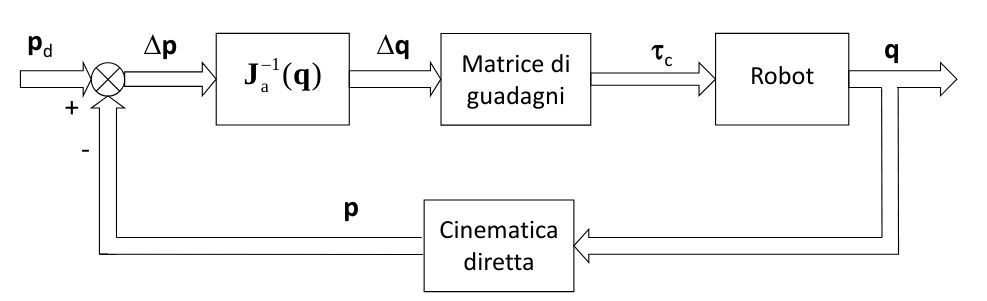
\includegraphics[width=0.7\linewidth]{images/operational_space_control_inv_jac}
	\caption{Schema a Jacobiano inverso}
	\label{fig:operationalspacecontrolinvjac}
\end{figure}







\subsection{Controllo a Jacobiano trasposto}
Negli schemi a Jacobiano trasposto l’errore $\Delta p$ nello spazio operazionale viene direttamente moltiplicato per una matrice di guadagni.
L’uscita di tale blocco può essere considerata come la forza elastica generata da una molla generalizzata, la cui funzione è di ridurre o cancellare la deviazione $\Delta p$. In altre parole la forza risultante guida la punta operativa lungo una direzione tale ridurre $\Delta p$.\\
La forza elastica definita nello spazio operazionale viene quindi trasformata nella corrispondente coppia da applicare ai giunti per mezzo dello Jacobiano trasposto (secondo le relazioni della statica viste).

\begin{figure}[H]
	\centering
	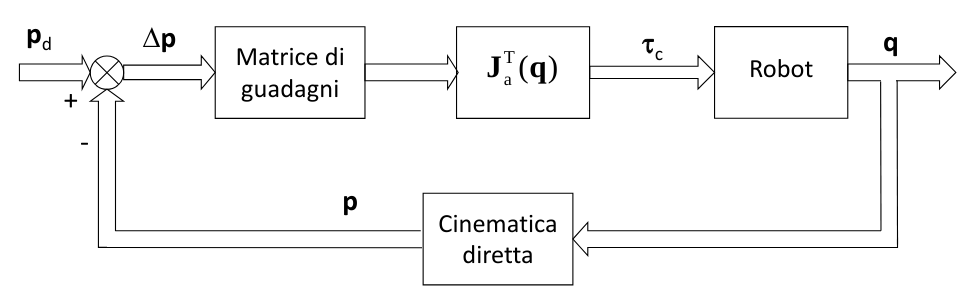
\includegraphics[width=0.7\linewidth]{images/operational_space_control_jac_trasp}
	\caption{Schema a Jacobiano trasposto}
	\label{fig:operationalspacecontroljactrasp}
\end{figure}


\textbf{Per questi schemi generali} (sia questo che quello a Jacobiano inverso) \textbf{non è né garantita la stabilità asintotica} né l’accuratezza di inseguimento della traiettoria, che dovranno essere assicurate dall’impiego di specifiche leggi di controllo, inserite in schemi dell’uno o dell’altro tipo.






\subsection{Controllo PD con compensazione della gravità}\label{section:pd_control_gravity_comp_join_space}
Vediamo nuovamente una tecnica di controllo PD con compensazione della gravità, questa volta però nello spazio operazionale.

Sia $p_d$ la posa costante desiderata per la punta operativa; \textbf{obiettivo} del controllo è \textbf{garantire} che \textbf{asintoticamente} si abbia $p_d - p = 0$.\\
È possibile dimostrare che tale richiesta è soddisfatta dalla legge di controllo:
\begin{equation}\label{eq:pd_gravity_comp_control_operational}
u = g(q) + J_A^T(q)(K_P(p_d - p) - K_DJ_A(q)\dot{q})
\end{equation}
costituita da una compensazione non lineare delle coppie di gravità, definita nello spazio dei giunti, e da una legge lineare di tipo PD definita nello spazio operazionale.

\vspace{5pt}
\subsubsection{Dimostrazione stabilità}
Con passaggi simili a quelli seguiti nello spazio dei giunti, si può dimostrare che il sistema raggiunge una postura di equilibrio asintoticamente stabile.
Partiamo nuovamente selezionando una funzione di Lyapunov (di nuovo $e \triangleq p_d - p$):
$$
V(\dot{q}, e) = \frac{1}{2}\dot{q}^TB(q)\dot{q} + \frac{1}{2}e^TK_Pe > 0 \qquad \forall \dot{q},e \neq 0
$$
e analizziamone il segno:
$$
\dot{V} = \dot{q}^TB(q)\ddot{q} + \frac{1}{2}\dot{B}(q)\dot{q} + \dot{e}K_Pe = \dot{q}^TB(q)\ddot{q} + \frac{1}{2}\dot{B}(q)\dot{q} - \dot{q}^TJ_A^T(q)K_Pe
$$
dove abbiamo usato il fatto che $\dot{x}_d = 0 \ , \ \dot{x}=J_A(q)\dot{q} \implies \dot{e} = \dot{x}_d - \dot{x} = - J_A(q)\dot{q}$.
Raccogliendo, richiamando di nuovo la \textit{null-property} di $\dot{B}(q) - 2C(q, \dot{q})$ e sostituendo a $B(q)\ddot{q}$ la forma di esso fornito da (\ref{eq:pd_gravity_comp_dyn}), otteniamo:
$$
\dot{V} = -\dot{q}^TF\dot{q} + \dot{q}^T(u - g(q) - J_A^T(q)K_Pe)
$$
dove, se sostituiamo ad $u$ la forma del controllo di (\ref{eq:pd_gravity_comp_control_operational}), otteniamo:
$$
\dot{V} = -\dot{q}^TF\dot{q} - \dot{q}^TJ_A^T(q)K_DJ_A(q)\dot{q}
$$
% e possiamo vedere che, per qualsiasi traiettoria del sistema, $\dot{V} \leq 0$ e $\dot{V} = 0 \iff \dot{q} = 0$.

% sezione \ref{section:pd_control_gravity_comp_join_space}
